% This text is proprietary.
% It's a part of presentation made by myself.
% It may not used commercial.
% The noncommercial use such as private and study is free
% Nov. 2006
% Author: Sascha Frank 
% University Freiburg 
% www.informatik.uni-freiburg.de/~frank/
%
% additional usepackage{beamerthemeshadow} is used
%  
%  \beamersetuncovermixins{\opaqueness<1>{25}}{\opaqueness<2->{15}}
%  with this the elements which were coming soon were only hinted

\documentclass{beamer}
%\usepackage{beamerthemeshadow}
\usetheme{Amsterdam}
\usepackage[catalan]{babel}
\usepackage[utf8]{inputenc}
\usepackage{url}
\begin{document}
\title{Algorismes genètics aplicats a ciències de la vida}
\author{Raimon Grau Cuscó}
\date{\today}

\AtBeginSection[]
{
\begin{frame}
    \frametitle{Índex}
    \tableofcontents[currentsection]
\end{frame}
}

\frame{\titlepage} 

\frame{\frametitle{index}\tableofcontents} 

\section{Motivació} % (fold)
\label{sec:Motivacio}
\begin{itemize}
	\item hola
	\item nanana ananan
	\item adeu
\end{itemize}
% section Motivació (end)


\section{Introducció} % (fold)

\begin{frame}
	\begin{columns}[c]
		\column{0.5\textwidth}
		\framebox{
\includegraphics[height=0.9\textheight,width=0.9\textwidth]{images/StrangeLoop.jpg}}
		\column{0.5\textwidth}
		\begin{itemize}
			\item hola
				\pause
			\item matat
		\end{itemize}
	\end{columns}
\end{frame}

\begin{frame}
	\frametitle{Creuament}
	\begin{columns}[c]
		\column{0.5\textwidth}
		\framebox{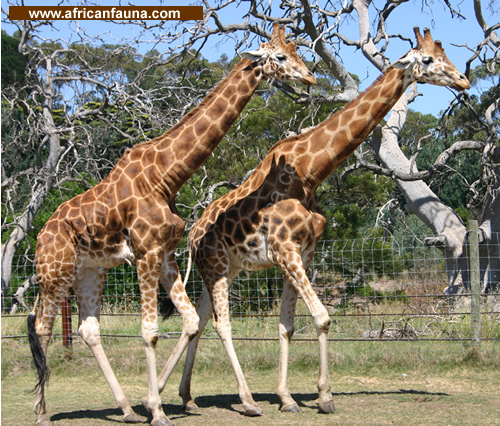
\includegraphics[height=0.7\textheight,width=0.9\textwidth]{images/giraffe-crossover.jpg}}
		\column{0.5\textwidth}
		\begin{itemize}
			\item 
				\pause
			\item matat
		\end{itemize}
	\end{columns}
\end{frame}

\begin{frame}
\end{frame}

\section{Algorismes evolutius} % (fold)
\label{sec:Algorismes evolutius}

% section Algorismes evolutius (end)

\section{Pholus} % (fold)
\label{sec:Pholus}
% section Pholus (end)

\section{Chiron} % (fold)
\label{sec:Chiron}
% section Chiron (end)

\section{GEP} % (fold)
\label{sec:GEP}
% section GEP (end)

\section{Conclusions} % (fold)
\label{sec:Conclusions}
\begin{frame}
	i tu ke tal
\end{frame}

\subsubsection{hola matat} % (fold)
\label{ssub:hola matat}
\begin{frame}
	jo bé
\end{frame}

% subsubsection hola matat (end)

% section Conclusions (end)


%\section{Objetivos y motivación} 
%\frame{\frametitle{Problemática} 
%Los hdd crecen y crecen, y nosotros no somos capaces de organizar toda la info
%\pause
%\begin{itemize}
%\item  Crear un programa de fácil interface, que permita moverme por mi hdd.
%\item  Funciona en X, para cualquier wm.
%\item  Tiene las mínimas dependencias posibles.
%\item  Tiene que ser 'intuitivo' para los usuarios (DWIM)
%\item  Tiene que ser extensible (a mas o menos nivel)
%\end{itemize}
%}

%\frame{\frametitle{¿Qué aplicaciones existen?}
%\begin{itemize}
%\item  Beagle \\
%Daemons!!
%\pause
%\item  Catfish \\
%- Mala interficie y limitado en configuracion. \\
%+ puede usar varios backends
%\pause
%\item  Google Desktop \\
%Linux?
%\pause
%\end{itemize}
%}

%\frame{\frametitle{Requerimientos}
%\begin{itemize}
%\item  Permite buscar y abrir archivos rápidamente
%\item  Ejecuta aplicaciones
%\item  Busca archivos remotamente
%\item  Permite gestionar playlists
%\item  Ayuda a navegar por las ventanas abiertas
%\item  No requiere utilizar ningún módulo ni ningun gestor de ventanas para funcionar (no todas las funcionalidades estaran activas)
%\item  Mínima heurística para facilitar su uso
%\end{itemize}
%}

%\section{Aproximación} 
%\subsection{Primera Aproximación}
%\frame{\frametitle{Buscando Ayudita}
%\begin{block}{find}
%find \~/ -name ``.*\$1.*''
%\end{block}
%\pause
%\begin{block}{ find2perl }
%find2perl [paths] [predicates] \textbar perl
%\end{block}
%}

%\begin{frame}[fragile]
%\frametitle{Buscando Ayudita(II)}
%\begin{block}{File::Find}
%\begin{verbatim}
%use File::Find; 
%find(\&wanted, @directories_to_search); 
%sub wanted { ... }
%\end{verbatim}
%\end{block}
%\pause
%\begin{block}{find2perl}
%\begin{verbatim}
%* File::Find::Rule
%# find all the .pm files in @INC
%my @files = File::Find::Rule->file()
%->name( '*.pm')
%->in(@INC);
%\end{verbatim}
%\end{block}
%\end{frame}

%\begin{frame}[fragile]
%\frametitle{¿Buscamos cada vez?}
%\begin{block} {File::Locate}
%\begin{verbatim}
%use File::Locate;
%print join "\n", locate "^/usr", 
%-rex => 1, "/usr/var/locatedb";
%\end{verbatim}
%\end{block}
%\pause
%\begin{block} {File::Locate::Harder}
%\begin{verbatim}
%my $flh = File::Locate::Harder->new( db => $db_file );
%my $results_aref = $flh->locate( $search_pattern,
%{ case_insensitive => 1,
%regexp => 1, });
%\end{verbatim}
%\end{block}
%\end{frame}

%\begin{frame}[fragile]
%\frametitle{¿Qué escojemos?}
%\pause
%\begin{center}
%\Huge{NINGUNA} \\
%\pause
%\Large{Portabilidad (GetOpt::Long; Pod::Usage)} \\
%\begin{verbatim}
%slocate -d $dbname $caseflag -r 
%".*$pattern[^/]*\.$ft\$"
%\end{verbatim}
%\end{center}
%\end{frame}


%\subsection{Interfeisss}
%\frame{
%\frametitle{Interfícies}
%\begin{block}{Tk}
%Complicado \\
%No standard
%\end{block}
%\pause
%\begin{block}{Zenity}
%zenity --info --text=``JAPH'' \\
%zenity --list --print-column 2 --hide-column 2 label out
%\end{block}
%\pause
%\begin{block}{ratmen}
%\$ENV\{RATPOISON\} -c `` echo YAPH ''  \\
%ratmen etiqueta1 comando1 etiqueta2 comando2
%\end{block}
%}

%\section{Código} 
%\begin{frame}
%\frametitle{Algoritmo}
%\begin{itemize}
%\item Checkear archivo de configuración
%\item Preguntar por una extensión/comando/orden
%\begin{itemize}
%\item si es extensión, pedir un patrón.
%\item si es una aplicación, ejecutarla
%\item si es una orden, ejecutarla. (gen, ff, vi)
%\end{itemize}
%\item Si es una extensión nueva pedimos una aplicación con la que abrir esos archivos.    
%\end{itemize}
%\begin{center}
%Usamos prefijos para distinguir entre .tex (archivo) y tex(aplicación)
%\end{center}
%\end{frame}

%\begin{frame}
%\frametitle{Prefijos y heurística}
%\begin{itemize}
%\item  .extensión
%\item -ejecutable
%\item ,ventana
%\pause
%\item Si no ponemos ningún prefijo, y entramos una extensión conocida, rf lo interpreta como EXTENSION.
%\item Si no es conocida y es un comando, se ejecuta el comando
%\item Si no es conocida y no es ningun comando, se agrega como nueva extensión
%\end{itemize}
%\end{frame}

%\begin{frame}[fragile]
%\frametitle{Recordar Extensiones}
%\begin{verbatim}
%lastft: pdf
%pdf xpf
%java gvim -f
%chm kchmviewer
%mp3 mocp -c -p -a
%\end{verbatim}
%\pause
%\begin{exampleblock}{Mejora}
%Pasarlo a codigo perl, y organizarlo como un hash, pudiendo
%hacer referencias a otras entradas: \\
%\$ext{ebook}=qw/pdf chm/; \$ext{chm}='kchmviewer';... 
%\end{exampleblock}
%\end{frame}

%\begin{frame}
%\frametitle{Flags}
%El usuario tiene que poder usar el programa sin tocar ni una linea de código.
%\begin{itemize}
%\item --all
%\item --case
%\item --conffile
%\item --loop (not implemented)
%\item --man
%\item --menuexe
%\item --remote
%\item --rootdir
%\end{itemize}
%\pause
%\begin{center}
%\large{GetOpt::Long y posibilidad de meter flags ``en vivo''}
%\end{center}
%\end {frame}

%\begin{frame}[fragile]
%\frametitle{GRID::Machine}
%El usuario puede definir una lista de servers donde tiene clave ssh SIN
%passphrase.
%\begin{verbatim}
%if ( $remote && eval{require GRID::Machine}){
%foreach (@remoteHosts){
%$m = GRID::Machine->new( host => $_ );
%for my $file (searchRemote($_,qq{slocate ... }, $m)){
%$file =~ m/.*\/(.*)$/;
%push @FileList, {path => $file ,name => "$1",
%machine => $m, IP => $_, app => ''};
%}
%}
%}
%\end{verbatim}
%\end{frame}


%\begin{frame}[fragile]
%\frametitle{GRID::Machine (II)}
%\begin{small}
%\begin{verbatim}
%$FileList[$res]{'machine'}->get(
%[$FileList[$res]{'path'}], '/tmp/');
%$^T = time();
%system($application. ' ' .quotemeta("/tmp". 
%"/$FileList[$res]{'name'}"));
%my $age = -M quotemeta("/tmp"."/$FileList[$res]{'name'}");
%$FileList[$res]{'path'} =~ s/(.*\/)[^\/]*/$1/mig;
%if ($^T == $age) {
%$FileList[$res]{'machine'}->put(["/tmp
%/$FileList[$res]{'name'}"],
%qq{$FileList[$res]{'path'}});
%}
%\end{verbatim}
%\end{small}
%\end{frame}

%\begin{frame}[fragile]
%\frametitle{Identificar paths con ``tilde''}
%\begin{verbatim}
%--rootdir=~/
%--rootdir=~foo
%--rootdir=~foo/bar

%$ext_app_file =~ s{ ^ ~ ( [^/]* ) }
%{ $1
%? (getpwnam($1))[7]
%: ( $ENV{HOME} || $ENV{LOGDIR}
%|| (getpwuid($>))[7]
%)
%}ex;
%\end{verbatim}
%\end{frame}

%\section{Un entorno de trabajo completo}
%\subsection{plugins}
%\begin{frame}[fragile]
%\frametitle{Define con WWW::Dictionary}
%\begin{verbatim}
%WWW::Dictionary;
%my $dictionary = WWW::Dictionary->new();
%my $meaning = $dictionary->meaning( $word );
%\end{verbatim}
%\pause
%\begin{verbatim}
%use WWW::Dictionary;
%my $dictionary = WWW::Dictionary->new( join('', @ARGV) );
%@_ = split ('\n' , $dictionary->get_meaning);
%print grep {/Spanish/} @_ , "\n";
%\end{verbatim}
%\end{frame}

%\begin{frame}[fragile]
%\frametitle{Syntax con WWW::Mechanize}
%HTML::Strip - Perl extension for stripping HTML markup from text
%\begin{verbatim}
%use WWW::Mechanize;
%use HTML::Strip;

%$w1 = WWW::Mechanize->new;
%$w1->get("http://www.google.es/search....");
%$html = HTML::Strip->new;
%$html->parse($w1->content);
%$html =~ m/de aproximadamente ([\d.]+) paginas/;
%\end{verbatim}
%\end{frame}


%\begin{frame}
%\frametitle{Trabajo Futuro}
%\begin{itemize}
%\item Refactorizar código
%\item Utilizar sqlite para localizar archivos.
%\item hacer 'plugins' para buscar streamings de música
%\item --loop flag
%\item --tmpcmd flag
%\end{itemize}
%\end{frame}

%\begin{frame}
%\frametitle{Bibliografia}	
%\begin{itemize}
%\item \url{http://software.twotoasts.de/?page=catfish}
%\item \url{http://beagle-project.org/Main\_Page}
%\item \url{www.cpan.org}
%\item O'Reilly Perl  Bookshelf (Beginning Perl,  Programming  Perl, Perl Cookbook...) 
%\item \url{http://use.perl.org/~Alias/journal/36415}
%\end{itemize}
%\end{frame}

%\begin{frame}
%Gracias por su atención
%\huge{\centering{http://code.google.com/p/ratfinder/}}
%\end{frame}


\end{document}
